\section{Dependencies}
\label{sec:depend}

Python has a well developed ecosystem of modules and packages to perform advanced tasks.
The modules listed below are used in this implementation.
\bigskip
 
\textit{optparse} [\url{https://docs.python.org/2/library/optparse.html}] \linebreak
The Python option parser \textit{optparse} is used to parse and set defaults for commandline options.
\bigskip

\textit{scipy} [\url{https://www.scipy.org/}]\linebreak
\textit{Scipy} is a widely used Python package for scientific computation. The linear algebra submodule \textit{linalg} is used in particular to implement the solver \ref{sec:solver} routine that solves the system of linear equations descirbing the system.
\bigskip

\textit{numpy} [\url{https://www.numpy.org/}]\linebreak
\textit{Numpy} is part of the \textit{scipy} package. Apart from the powerful N-dimensional array object used to implement the matrices and vectors several trigonometric functions were used because they are often faster, more stable than the Python math functions and can perform element-wise operations.
\bigskip

\textit{matplotlib} [\url{https://matplotlib.org/}]\linebreak
\textit{Matplotlib} is a powerful Python plotting library. It is used to visualize the system geometry, load vectors, stress resultants and an approximated deflection plot using B\'{e}zier curves.
\bigskip

\textit{csv} [\url{https://docs.python.org/2/library/csv.html}]\linebreak
The \textit{csv} module implements classes to read and write so-called CSV (Comma Separated Values) format spreadsheets used for human readable as well as computer generatable input of system geometry, load vectors, material and profile values, and constraints.
It is also used to store the results (displacement vectors and resultant stresses) of the computation.

\pagebreak

\section{Source Code Files}
\label{sec:srcfiles}

The program is split into multiple modules containing different functions described later in this chapter.

\subsection{main.py}
\label{subsec:main.py}

The main module calls the functions from the different modules and first perfoms the option parsing.

\begin{inconsolata}
\begin{lstlisting}[language=python]
...
def main():

    parser = OptionParser(usage="usage: %prog [options]",
                          version="%prog " + str(version))

    # Input Files                                       

    group = OptionGroup(parser, "Input files")

    group.add_option("-N", "--NodeFile",
                     type="string",
                     action="store",
                     dest="nodeFile",
                     default='Input_nodes.csv',
                     help="CSV file with node definitions")
...
\end{lstlisting}
\end{inconsolata}

After parsing the command line options the CSV input files for node, strut, constraint and load definitions are loaded respectively.
Nodes not referenced by any strut (free nodes) are deleted.

\begin{inconsolata}
\begin{lstlisting}[language=python]
...
    nodes       = readCSV(options.nodeFile,
                          nodesTypeTemplate)

    struts      = readCSV(options.strutFile,
                          strutsTypeTemplate)

    deleteFreeNodes(nodes, struts)

    constraints = readCSV(options.constFile,
                          constraintTypeTemplate)

    strutLoads  = readCSV(options.strutLoadFile,
                          strutLoadTypeTemplate)

    nodeLoads   = readCSV(options.nodeLoadFile,
                          nodeLoadTypeTemplate)
...
\end{lstlisting}
\end{inconsolata}

\pagebreak

To validate the references several checks are performed on the data.

\begin{inconsolata}
\begin{lstlisting}[language=python]
...
    checkStrutNodes(nodes, struts)
    checkConstraintNodes(nodes, constraints)
    checkStrutLoads(struts, strutLoads)
    checkNodeLoads(nodes, nodeLoads)
...
\end{lstlisting}
\end{inconsolata}

Properties that can be derived from the inputs (length, angle, type and local member force vector $S\textsubscript{L}$ resulting from the strut loads) and are needed for later computations are calculated and stored in the strut objects.

\begin{inconsolata}
\begin{lstlisting}[language=python]
...
    getStrutLength(nodes, struts)
    getStrutAngle(nodes, struts)
    getStrutType(struts)
    assemble_S_L(strutLoads, struts, nodes)
...
\end{lstlisting}
\end{inconsolata}

The global force vector $S\textsubscript{G}$ is then calculated from node loads and strut loads.

\begin{inconsolata}
\begin{lstlisting}[language=python]
...
    S_G = assemble_S_G(nodeLoads, struts, nodes)
...
\end{lstlisting}
\end{inconsolata}

The system stiffness matrix $K$ is then assembled from the stiffness matrices $K\textsubscript{i}$ of the the individual struts and constraints are applied.

\begin{inconsolata}
\begin{lstlisting}[language=python]
...
    K = assemble_global_K_I(nodes, struts)
    apply_constraints(K, struts, nodes, constraints)
...
\end{lstlisting}
\end{inconsolata}

Now checks can be performed if the system is kinematic. The two criteria used here are:
\begin{itemize}

  \item Underdefined system (not enough constraints)

\begin{equation}
n < 3
\end{equation}

  \item The system stiffness matrix has a non-trivial solution

\begin{equation}
det K = 0
\end{equation}

\end{itemize}

\begin{inconsolata}
\begin{lstlisting}[language=python]
...
    if sp.det(K) == 0:
        print('System is kinematic (det(K)=0)!')
        exit()

    if countConst(constraints) < 3:
        print('System is kinematic (n < 3)!')
        exit()
...
\end{lstlisting}
\end{inconsolata}

If these checks are passed the solver can be called to calculate the displacement vector $d$.
After obtaining $d$ the resulting local member forces $S\textsubscript{L}$ can be calculated and stored in the corresponding strut objects.

\begin{inconsolata}
\begin{lstlisting}[language=python]
...
    d = solver(K, S_G, constraints, nodes)
    calc_local_forces(nodes, struts, d)
...
\end{lstlisting}
\end{inconsolata}

Now that the analysis is complete the output can be written to a CSV file and a function called to visualize the system geometry, loads, displacement, deflection and stress resultants.

\begin{inconsolata}
\begin{lstlisting}[language=python]
...
    writeDisplacements(options.displacementVectorFile,
                       d,
                       nodes)
    drawSystem(nodes,
               struts,
               constraints,
               strutLoads,
               nodeLoads,
               d,
               float(options.scale),
               options.savePlot)
...
\end{lstlisting}
\end{inconsolata}


\subsection{util.py}
\label{subsec:util.py}

The utility module contains small helper functions used in all other modules.
These mostly deal with traversing Python's data structures relating names and ids of strut and node objects but also formatting matrices and object properties for debugging output.

\subsection{input\_templates.py}
\label{subsec:inputtemplates.py}

In order to generate parsers for the CSV input files a template is needed which contains attribute names and type information.

\begin{inconsolata}
\begin{lstlisting}[language=python]
...
strutsTypeTemplate      = [ ('ID' , str),
                            ('StartNode' , str),
                            ('StartHinge' , int),
                            ('EndNode' , str),
                            ('EndHinge' , int),
                            ('E' , float),
                            ('A' , float),
                            ('I' , float)]
...
\end{lstlisting}
\end{inconsolata}

\subsection{input.py}
\label{subsec:input.py}

\textit{input.py} contains the parser generators and type conversion functions used to convert the \textit{string} values from the CSV files to the desired types specified in the corresponding templates.
If conversion fails an error is thrown, telling the user where the malformed input is located.
The functions used to perform checks on the input and derive data used for further computation are also located in this module.

\begin{inconsolata}
\begin{lstlisting}[language=python]
...
def typeConv(_dict, _typeTemplate):...
def readCSV(csvFile, typeTemplate):...
def genTemplate(filename, typeTemplate):...
def checkStrutNodes(nodes, struts):...
def checkConstraintNodes(nodes, constraints):...
def checkStrutLoads(struts, strutLoads):...
def checkNodeLoads(nodes, nodeLoads):...
def deleteFreeNodes(nodes, struts):...
def getStrutLength(nodes, struts):...
def getStrutAngle(nodes, struts):...
def getStrutType(struts):...
def strutLength(strut, nodes):...
def strutAngle(strut, nodes):...
def strutType(strut):...
\end{lstlisting}
\end{inconsolata}

\subsection{output.py}
\label{subsec:output.py}

The functions of the \textit{output} module are used to convert and store the results of the analysis in CSV files.

\subsection{solver.py}
\label{subsec:solver.py}

The \textit{solver} module implements the routine to solve the system of linear equations using methods form the \href{http://www.netlib.org/lapack/}{LAPACK} package contained in \textit{scipy}:

\begin{equation}
S\textsubscript{G} = K * d
\end{equation}

After computing the solution the constraints are apllied to the resulting vector $d$.

\begin{inconsolata}
\begin{lstlisting}[language=python]
...
def solver(K, S_G, constraints, nodes):
    d = sp.solve(K,S_G)

    #apply constraints: set d[i] = 0
    for ID, const in constraints.iteritems():
        id = nodeNameToID(const['Node'], nodes)
        if const['x']:
            x = id * 3
            d[x] = 0
        if const['z']:
            x = id * 3 + 1
            d[x] = 0
        if const['r']:
            x = id * 3 + 2
            d[x] = 0

    return d
\end{lstlisting}
\end{inconsolata}

\subsection{load\_vectors.py}
\label{subsec:loadvectors.py}

This module encompasses all function definitions to calculate the local member forces $S\textsubscript{L}$ \note{Add bib ref to Schneider tables} resulting from the different load vectors \ref{fig:loadVec} for each member type \ref{fig:memberTypes}.


\begin{figure}[h]%
    \centering
    \subfloat[Type 1: trapazoid]{{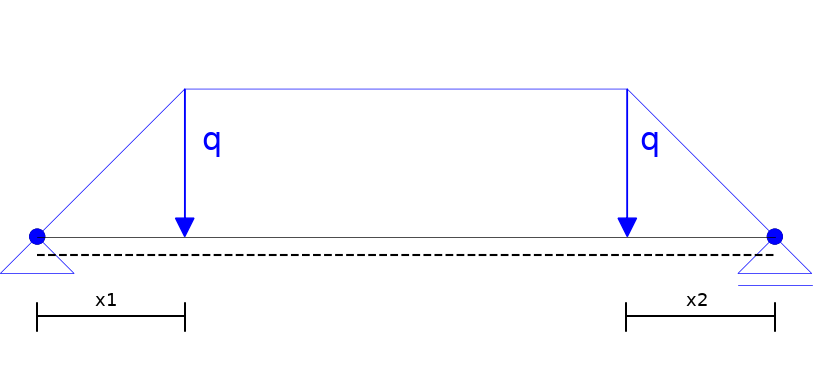
\includegraphics[width=0.4\textwidth]{load_type_1.png}}}%
    \qquad
    \subfloat[Type 2: torque]{{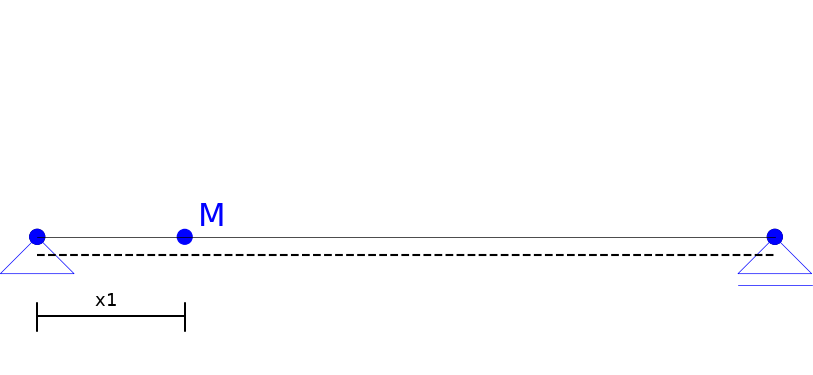
\includegraphics[width=0.4\textwidth]{load_type_2.png}}}%

    \centering
    \subfloat[Type 3: force]{{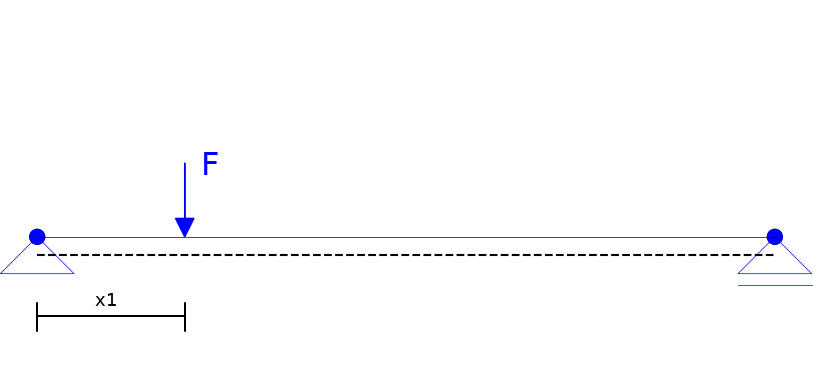
\includegraphics[width=0.4\textwidth]{load_type_3.png}}}%
    
    \caption{Load Vectors}%
    \label{fig:loadVec}%
\end{figure}


\begin{figure}[h]%
    \centering
    \subfloat[Type 1: both joints rigid]{{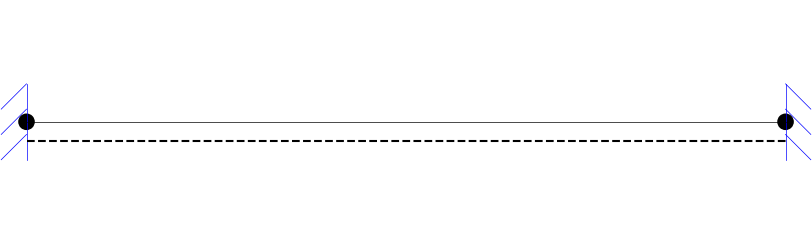
\includegraphics[width=0.4\textwidth]{strut_type_1.png}}}%
    \qquad
    \subfloat[Type 2a: right: pin-jointed, left: rigid joint]{{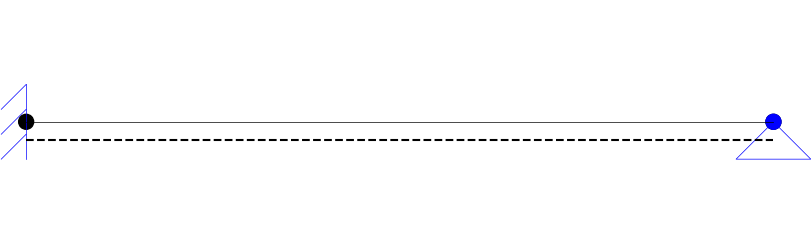
\includegraphics[width=0.4\textwidth]{strut_type_2a.png}}}%

    \centering
    \subfloat[Type 2b: right: rigid joint, left: pin-jointed]{{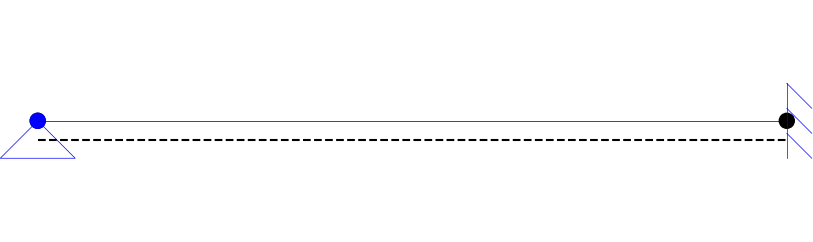
\includegraphics[width=0.4\textwidth]{strut_type_2b.png}}}%
    \qquad
    \subfloat[Type 3: both pin-jointed]{{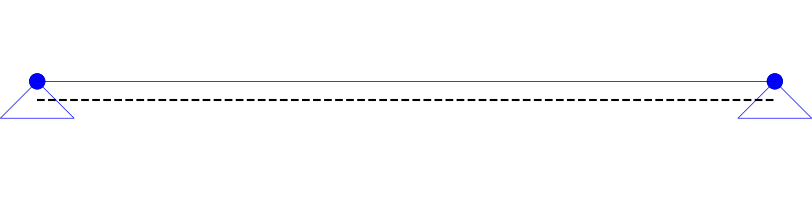
\includegraphics[width=0.4\textwidth]{strut_type_3.png}}}%
    
    \caption{Member Types}%
    \label{fig:memberTypes}%
\end{figure}

\begin{inconsolata}
\begin{lstlisting}[language=python]
...
def S_L_1_1( x1, x2, l, F, M, q ):...
def S_L_1_2a( x1, x2, l, F, M, q ):...
def S_L_1_2b( x1, x2, l, F, M, q ):...
def S_L_1_3( x1, x2, l, F, M, q ):...

def S_L_2_1( x1, x2, l, F, M, q ):...
def S_L_2_2a( x1, x2, l, F, M, q ):...
def S_L_2_2b( x1, x2, l, F, M, q ):...
def S_L_2_3( x1, x2, l, F, M, q ):...

def S_L_3_1( x1, x2, l, F, M, q ):...
def S_L_3_2a( x1, x2, l, F, M, q ):...
def S_L_3_2b( x1, x2, l, F, M, q ):...
def S_L_3_3( x1, x2, l, F, M, q ):...
...
\end{lstlisting}
\end{inconsolata}

The function references are stored in a \textit{dictionary} and dereferenced by member and load type as keys to simplify the implementation of the \textit{get\_S\_L} function and allow for easy expandability.

\begin{inconsolata}
\begin{lstlisting}[language=python]
...
dict = {
    1:{
        '1'  : S_L_1_1,
        '2a' : S_L_1_2a,
        '2b' : S_L_1_2b,
        '3'  : S_L_1_3
    },
    2:{
        '1'  : S_L_2_1,
        '2a' : S_L_2_2a,
        '2b' : S_L_2_2b,
        '3'  : S_L_2_3
    },
    3:{
        '1'  : S_L_3_1,
        '2a' : S_L_3_2a,
        '2b' : S_L_3_2b,
        '3'  : S_L_3_3
    }
}

#calculates the load vector from a load
def get_S_L( load, strut):
    x1 = load['x1']
    x2 = load['x2']
    l  = strut['l']
    F  = load['F']
    M  = load['M']
    q  = load['q']
    loadType = load['Type']
    strutType = strut['Type']

    return dict[loadType][strutType](x1, x2, l, F, M, q)
...
\end{lstlisting}
\end{inconsolata}

A function to assemble the global load vector $S\textsubscript{G}$ from the local member forces $S\textsubscript{L}$ by rotating them to global coordinates ($S\textsubscript{G} = S\textsubscript{L} * rot(\alpha)$ \ref{rot}) and the node loads by simply adding them to the vector is also part of the module.

\begin{equation} \label{rot}
rot = \begin{pmatrix}
cos(\alpha)  & sin(\alpha)  & 0   & 0             & 0             & 0   \\[0.2em]
-sin(\alpha) & cos(\alpha)  & 0   & 0             & 0             & 0   \\[0.2em]
0            & 0            & 1   & 0             & 0             & 0   \\[0.2em]
0            & 0            & 0   & cos(\alpha)   & sin(\alpha)   & 0   \\[0.2em]
0            & 0            & 0   & -sin(\alpha)  & cos(\alpha)   & 0   \\[0.2em]
0            & 0            & 0   & 0             & 0             & 1
     \end{pmatrix}
\end{equation}

\begin{inconsolata}
\begin{lstlisting}[language=python]
...
#creates the global load vector from strut loads and node loads
def assemble_S_G( nodeLoads, struts, nodes ):
    size = len(nodes) * 3
    S_G = np.zeros(size)

    #add node loads
    for ID, load in nodeLoads.iteritems():
        id = nodeNameToID(load['Node'], nodes)
        Fx = load['Fx']
        Fz = load['Fz']
        M  = load['M']
        v = np.array([Fx, Fz, M])
        for i in range(3):
            S_G[id*3 + i] += v[i]

    #add strut load vectors
    for ID, strut in struts.iteritems():
        id = nodeNameToID(strut['StartNode'], nodes)

        S_L = np.zeros(6)
        if 'S_L' in strut:
            S_L = strut['S_L']

        #rotate to global coordinates
        alpha = strut['alpha']
        v = rot(alpha).dot(S_L)
        for i in range(6):
            S_G[id*3 + i] += v[i] * -1

    return S_G
...
\end{lstlisting}
\end{inconsolata}

\subsection{matrices.py}
\label{subsec:matrices.py}

\textit{matrices} is used to deal with the required matrix operations and to calculate the matrices of the different member types \ref{fig:memberTypes}.

\begin{equation} \label{K1}
K\textsubscript{1} = \begin{pmatrix}
\dfrac{EA}{l} & 0                   & 0                   & -\dfrac{EA}{l}  & 0                   & 0                   \\[0.8em]
              & 2d\dfrac{EI}{l^3}   & -d\dfrac{EI}{l^2}   & 0               & -2d\dfrac{EI}{l^3}  & -d\dfrac{EI}{l^2}   \\[0.8em]
              &                     & a\dfrac{EI}{l}      & 0               & d\dfrac{EI}{l^2}    & b\dfrac{EI}{l}      \\[0.8em]
              &                     &                     & 0               & \dfrac{EA}{l}       & 0                   \\[0.8em]
              &                     &                     &                 & 0                   & d\dfrac{EI}{l^2}    \\[0.8em]
              &                     &                     &                 &                     & a\dfrac{EI}{l}
     \end{pmatrix}
\end{equation}

\begin{equation} \label{K2a}
K\textsubscript{2a} = \begin{pmatrix}
\dfrac{EA}{l} & 0                   & 0                   & -\dfrac{EA}{l}  & 0                   & 0                   \\[0.8em]
              & c\dfrac{EI}{l}      & -c\dfrac{EI}{l^2}   & 0               & -\dfrac{EI}{l^3}    & 0                   \\[0.8em]
              &                     & c\dfrac{EI}{l}      & 0               & c\dfrac{EI}{l^2}    & 0                   \\[0.8em]
              &                     &                     & \dfrac{EA}{l}   & 0                   & 0                   \\[0.8em]
              &                     &                     &                 & c\dfrac{EI}{l^3}    & 0                   \\[0.8em]
              &                     &                     &                 &                     & 0
     \end{pmatrix}
\end{equation}

\begin{equation} \label{K2b}
K\textsubscript{2b} = \begin{pmatrix}
\dfrac{EA}{l} & 0                   & 0                   & -\dfrac{EA}{l}  & 0                   & 0                   \\[0.8em]
              & \dfrac{EI}{l^3}     & 0                   & 0               & -c\dfrac{EI}{l^3}   & -c\dfrac{EI}{l^2}   \\[0.8em]
              &                     & 0                   & 0               & 0                   & 0                   \\[0.8em]
              &                     &                     & \dfrac{EA}{l}   & 0                   & 0                   \\[0.8em]
              &                     &                     &                 & c\dfrac{EI}{l^3}    & c\dfrac{EI}{l^2}    \\[0.8em]
              &                     &                     &                 &                     & c\dfrac{EI}{l}
     \end{pmatrix}
\end{equation}

\begin{equation} \label{K3}
K\textsubscript{3} = \begin{pmatrix}
\dfrac{EA}{l} & 0                   & 0                   & -\dfrac{EA}{l}  & 0                   & 0                   \\[0.8em]
              & 0                   & 0                   & 0               & 0                   & 0                   \\[0.8em]
              &                     & 0                   & 0               & 0                   & 0                   \\[0.8em]
              &                     &                     & \dfrac{EA}{l}   & 0                   & 0                   \\[0.8em]
              &                     &                     &                 & 0                   & 0                   \\[0.8em]
              &                     &                     &                 &                     & 0
     \end{pmatrix}
\end{equation}

Stabkennzahl \note{English?!}

\begin{equation} \label{e}
\epsilon = l\sqrt{\frac{|N|}{EI}}
\end{equation}

The coeffecients $a, b, c ,d$ are functions in second order theory and model stiffening and weakening due to normal force.
In first order theory ($N = 0 \Rightarrow \epsilon = 0$) they are treated as constants.

\begin{equation} \label{a}
    a = \begin{cases}
            \hfil 4              & \text{if } \epsilon \leq 0\\[1.2em]
            \hfil \dfrac{\epsilon * sin(\epsilon) - \epsilon^2 * cos(\epsilon)}{2 * (1 - cos(\epsilon)) - (\epsilon * sin(\epsilon))}               & \text{if } N < 0          \\[1.2em]
            -\dfrac{\epsilon * sinh(\epsilon) - \epsilon^2 * cosh(\epsilon)}{2 * (1 - cosh(\epsilon)) + \epsilon * sinh(\epsilon)}               & \text{if } N > 0
        \end{cases}
\end{equation}

\begin{equation} \label{b}
    b = \begin{cases}
            \hfil 2              & \text{if } \epsilon \leq 0\\[1.2em]
            \hfil \dfrac{\epsilon^2 - sin(\epsilon)}{2*(1 - cos(\epsilon)) - \epsilon * sin(\epsilon) }               & \text{if } N < 0          \\[1.2em]
            -\dfrac{\epsilon^2 - \epsilon * sinh(\epsilon))}{2 * (1 - cosh(\epsilon)) + \epsilon * sinh(\epsilon)}               & \text{if } N > 0
        \end{cases}
\end{equation}

\begin{equation} \label{c}
    c = \begin{cases}
            \hfil 3              & \text{if } \epsilon \leq 0\\[1.2em]
            \hfil \dfrac{\epsilon^2 * sin(\epsilon)}{sin(\epsilon) - \epsilon * cos(\epsilon)}               & \text{if } N < 0          \\[1.2em]
            -\dfrac{\epsilon^2 * sinh(\epsilon)}{sinh(\epsilon) - \epsilon * cosh(\epsilon)}               & \text{if } N > 0
        \end{cases}
\end{equation}

\begin{equation} \label{d}
    d = a + b
\end{equation}

\begin{figure}[h]%
    \centering
    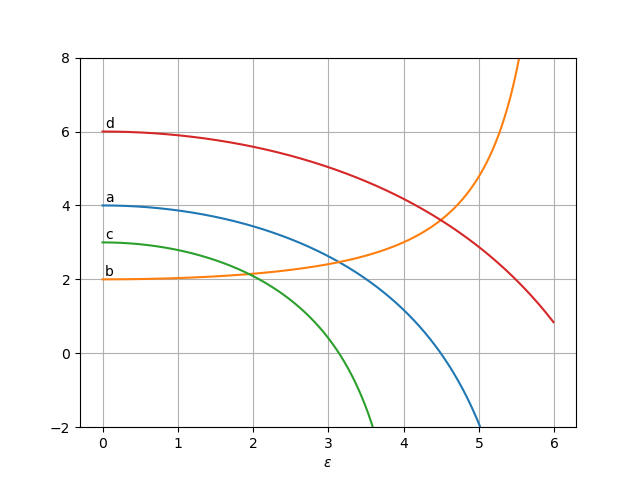
\includegraphics[width=0.9\textwidth]{coeff_N_neg.png}%
    \caption{Coefficients for negative normal pressure}%
    \label{fig:coeff_N_neg}%
\end{figure}

\begin{figure}[h]%
    \centering
    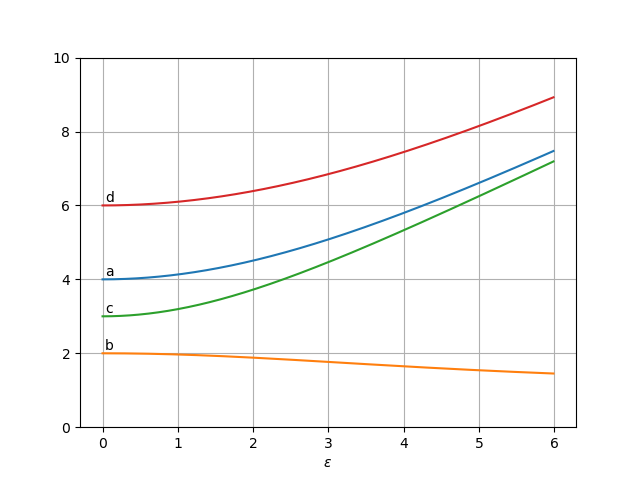
\includegraphics[width=0.9\textwidth]{coeff_N_pos.png}%
    \caption{Coefficients for positive normal pressure}%
    \label{fig:coeff_N_pos}%
\end{figure}

\begin{equation} \label{symmetrize}
    M\textsubscript{sym} = M + M^T - diag(M)
\end{equation}


\begin{inconsolata}
\begin{lstlisting}[language=python]
...
def symmetrize(M):
    return M + M.T - np.diag(M.diagonal())
...
\end{lstlisting}
\end{inconsolata}


\subsection{graphics.py}
\label{subsec:graphics.py}


\pagebreak

\section{Option Parsing}
\label{sec:optparse}


\section{Input Parsing}
\label{sec:inputpars}

\subsection{CSV Parser}
\label{sec:csvparse}

\subsection{Input Checking}
\label{sec:inputcheck}


\section{Assembling Matrices and Vectors}
\label{sec:asmmatrvec}

\subsection{Global Member Force Vector $S\textsubscript{G}$}
\label{sec:asmSG}
\subsection{System Stiffness Matrix $K$}
\label{sec:asmK}

\subsection{Applying Constraints}
\label{sec:applyconst}


\section{Checking for Kinematic System Conditions}
\label{sec:kinesyscheck}


\section{Solving the Resulting System of Linear Equations}
\label{sec:solver}
